
To evaluate the application's ability to meet user requirements, two rounds of user testing sessions were conducted at the DNV GL headquarters in Høvik, Norway.
The first of these session involved one test person, while the second session involved two. 
The participants were brought in individually and asked to take a seated position at an ordinary work station (i.e an office space) with a mouse, keyboard and display, 
in addition to a Leap Motion Controller positioned at the desk between the keyboard and the user. A HTC Vive head mount was also present for use during the experimentation phase. 
The computer used for the testing had the following specifications (hardware and software):

\begin{itemize}
    \item An Intel i7 as processor.
    \item 8 GB of RAM.
    \item A Nvidia Geforce GTX 1080 graphics card.
    \item A Windows 10 64-bit operating system (build 14393).
    \item Unity 5.5.2
    \item Leap Motion Control Panel version 3.2.0+45899
    \item Steam VR runtime (for use with the HTC Vive HMD)
\end{itemize}

\begin{figure}%[h!] %[H]
	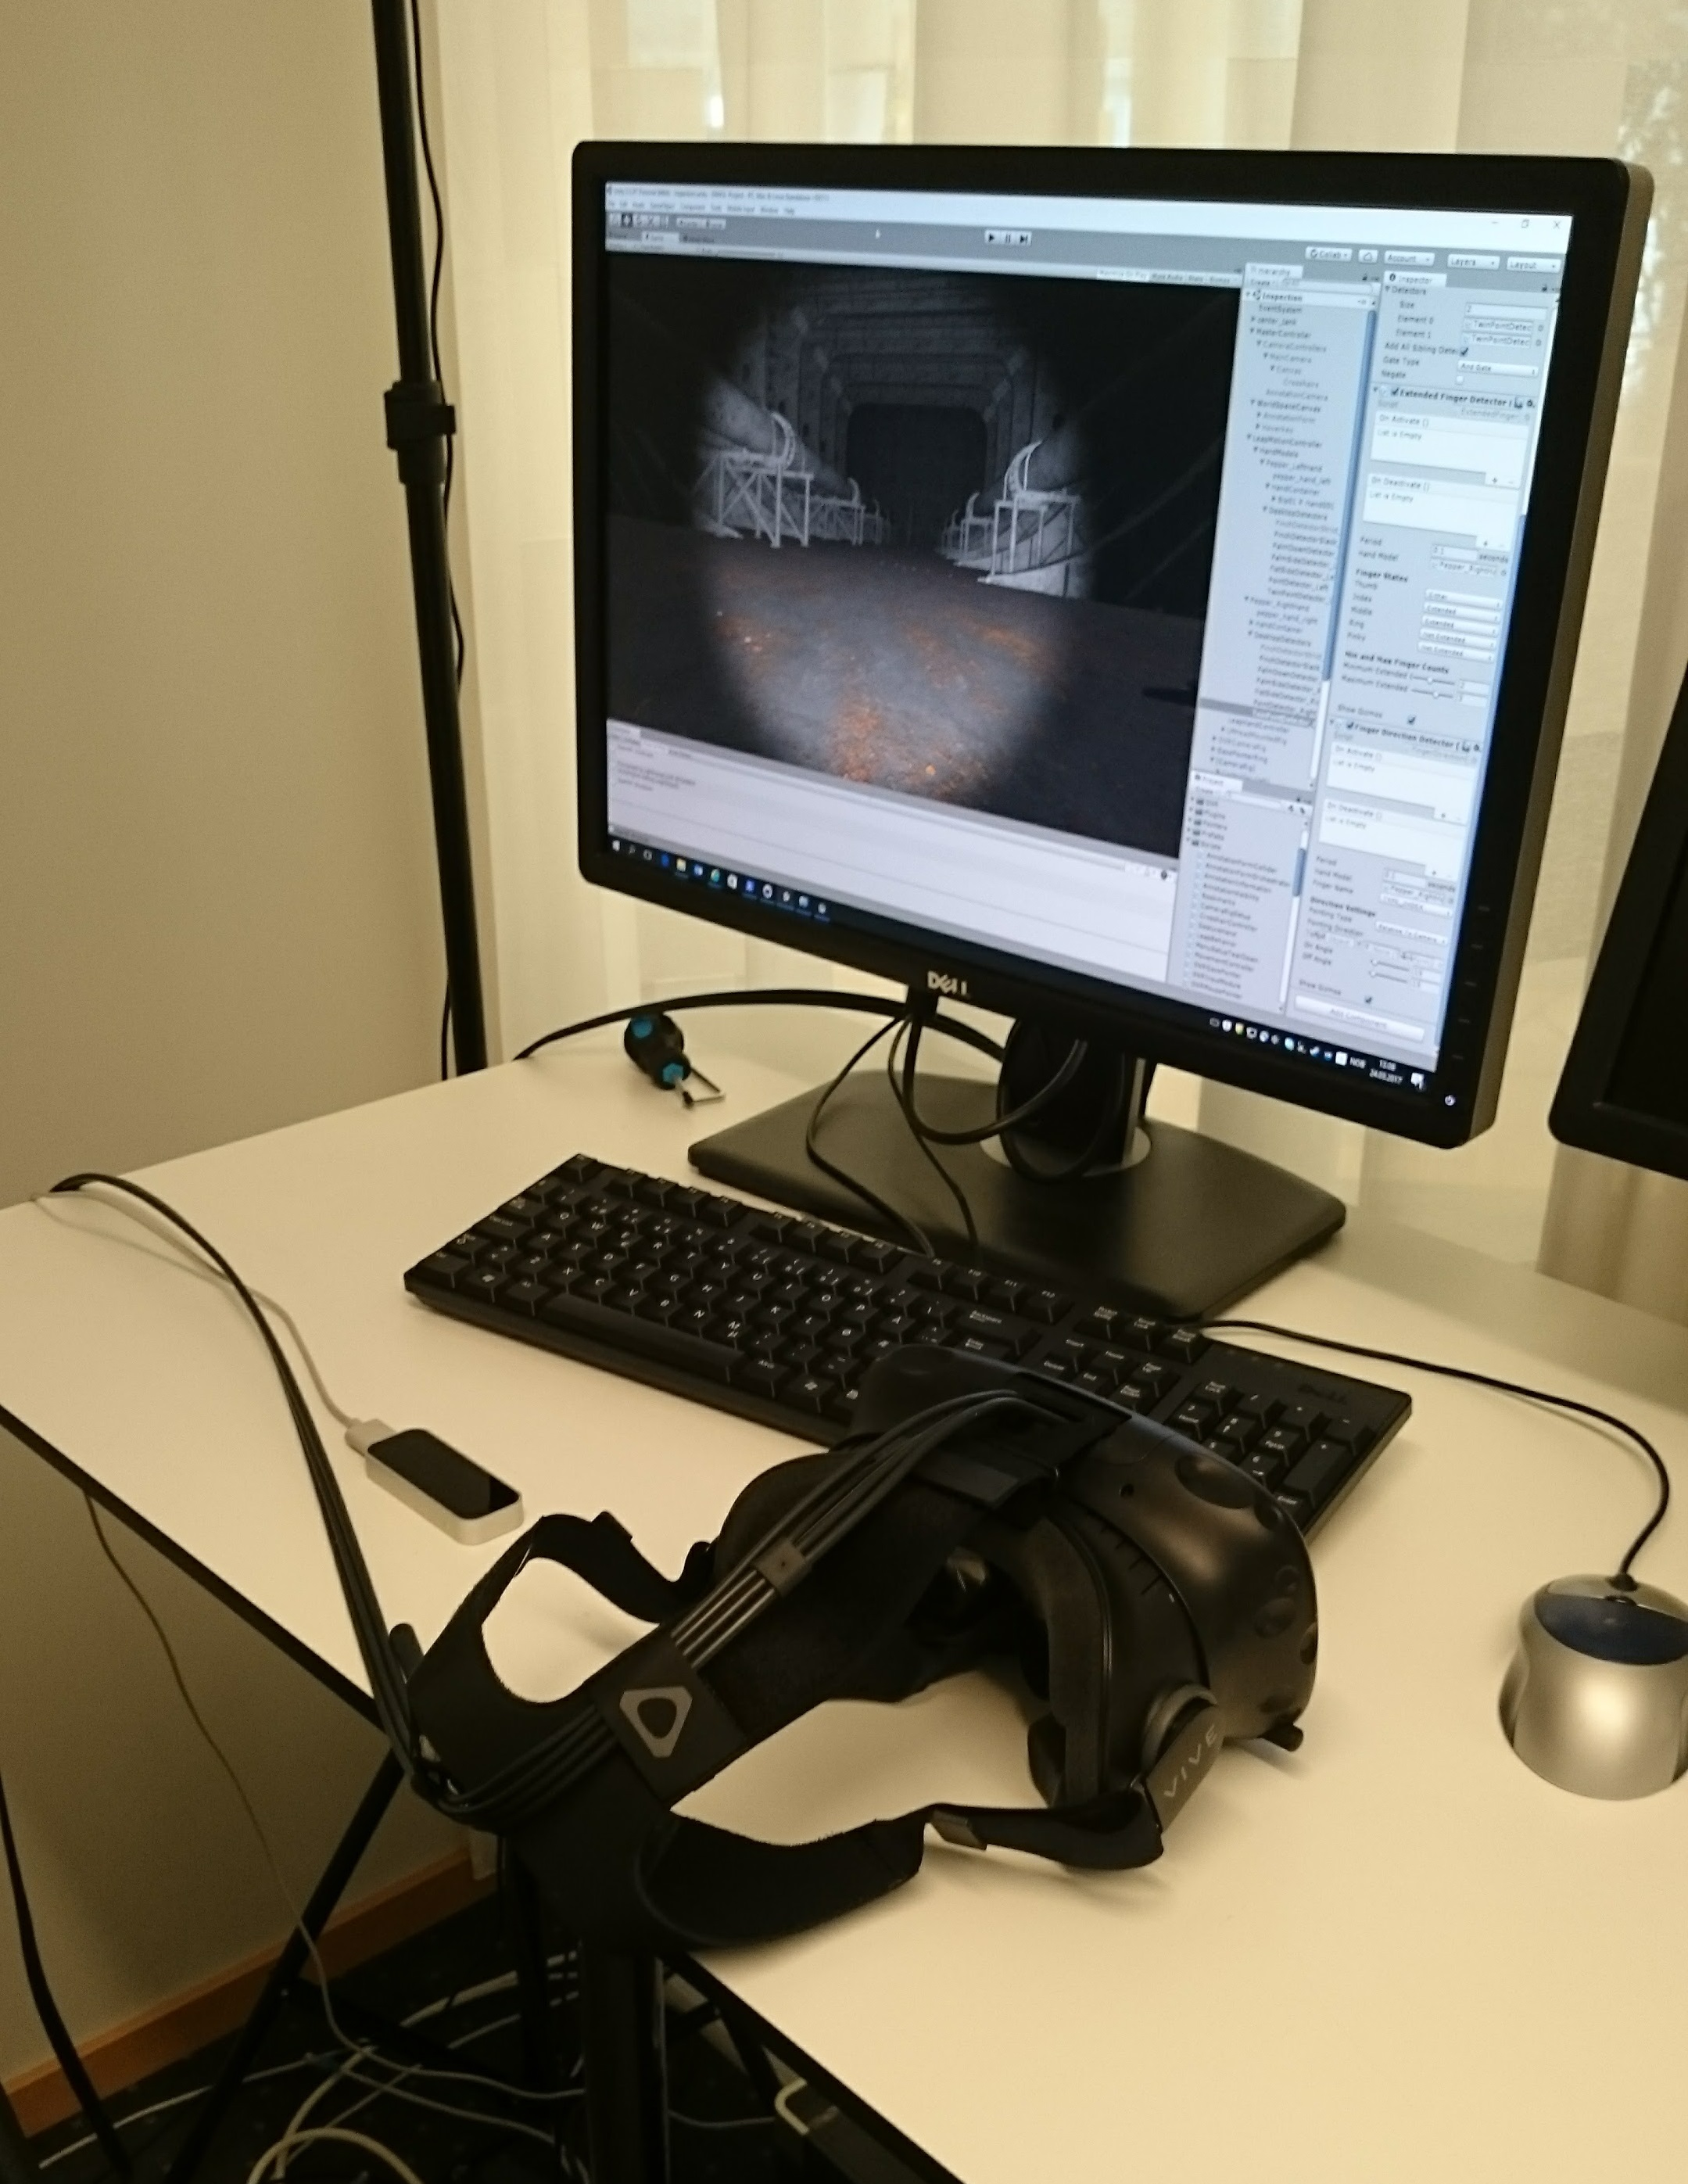
\includegraphics[width=\linewidth]{pictures/test_setup.jpg}
	\caption[The user test session setup.]{The user test session setup at DNV GL. }
	\label{fig:test_setup}
\end{figure} 

After the participant was seated the test phases were conducted in the following order (including an estimate of alloted time):

\begin{enumerate}
    \item  5 minutes of introduction. The users were informed about the purpose of the application, some of its long term goals and its limitations.
    \item 10 minutes of demonstration. The users were shown each of the possible actions and the different gestures available to them.
    \item 15 minutes of instructions. The users followed a series of instructions and oral explanations to teach them to use the program.
    \item 20 minutes of experimentation. The users were asked to use the program freely without any instructions.  
    \item 10 minutes of questions. The users were interviewed with a series of questions related to the application and their experience using it.   
\end{enumerate}

With the exception of the experimentation phase, all the steps above were conducted without the use of a virtual reality headset. 
This was done to more easily explain and show different gestures - which is easier when not wearing a HMD - and to allow the user to 
get familiar with the gesture scheme before using the virtual reality headset (to e.g.~~reduce the amount of unintended movements).
In the experimentation phase, the participants were asked to divide their time equally between using the application in \textit{desktop mode} 
- a collection of settings intended for usage with a regular display - and \textit{Virtual reality mode} - settings intended for usage with a virtual reality HMD. 

\section{The Instructions}
The participants were asked to perform the following tasks:

\begin{enumerate}
    \item The pinch gesture is performed by pushing the thumb and index finger together, while keeping the palm directed against the table surface. 
          Move the hand which holding the pinch gesture to rotate the camera along the X and Y axis.
    
    \item The Palm-down gesture (alternatively, the Y gesture) is performed by holding your hand straight with all fingers extended, pointing towards the screen and the palm facing downward towards the table surface. 
          Lift and lower your hand to change move the camera along the Y axis. 
    
    \item The Palm-side gesture (alternatively, the X gesture) is performed by holding your hand straight with all fingers extended, pointing towards the screen and the palm facing to the side, 
          perpendicular to the table surface. 
          Move it from side to side to move the camera along the X axis.
    
    \item The fist gesture (alternatively, the Z gesture) is performed by holding your hand curled up into a fist with no finger extended, pointing towards the screen and the palm facing downward towards the table surface. 
          Move your fist closer or further from the screen to move the camera along the Z axis. 
    
    \item Maneuver from your current position around one of the pipes present in the 3D model and back to your original position, using one or both hands. 
    
    \item Hold your left hand straight and rotate it so the palm if facing towards you. A menu shaped like a fan should appear and follow the movements of your left hand as long as
          this gesture is held. Use the index finger of the right hand to select "Toggle Options" and then "Combine XYZ Gestures". 
          To select a button hold the tip of the right index finger close enough (in terms of X, Y and Z axis) to the button for it to gradually highlight. 
          When "Combine XYZ Gestures" has been selected the X, Y and Z gestures are combined/replaced by a combined XYZ gesture, which is performed the same way as the Y gesture
          (hand straight and palm down). When now performing and holding this gesture the user can move along the X, Y, and Z axis in the virtual space by moving the hand 
          correspondingly in the physical space.

    \item Maneuver as in instruction \#5, but this time by using in the combined XYZ gesture. After the user has completed this s/he might switch back to the other gesture scheme
          by bringing up the menu and select "Toggle Option" and "Distinguish XYZ Gestures", or keep the the combined XYZ gesture.

    \item By utilizing the gestures introduced thus far, move the camera so the cursor/crosshair in the middle of the screen is positioned over a nearby object. 
          Perform a pointing gesture by only having the index finger extended and point at the screen (away from you). If this is done correctly a blue sphere should occur, which
          is called an "Annotation Sphere". This is in short a unit of information related to the position it is attached to. Create two more Annotation Spheres by moving the 
          cursor/crosshair over other nearby surfaces and point. 
    
    \item Now annotate/mark an entire object or surface by pointing two fingers ("double pointing") instead of one. These two fingers should ideally be held in a bit of an angle, like a scissor. 
          When done correctly the entire surface or object the cursor/crosshair is indicating should be colored in a similar blueish color as the annotation spheres. 

    \item Now place the cursor/crosshair over an annotation sphere or an annotated object and either point (if an annotation sphere is selected) or double point (if an annotated
          object is selected). When done correctly a form containing a text field, a virtual keyboard and some buttons should be displayed. 

    \item Write "DNV GL" in the text field by utilizing the virtual keyboard. After this click on one of the colored buttons to set a color on there annotation (used to indicate a 
          priority), and click submit to save the changes to the annotation. 

    \item Open the same annotation again by and delete it by pressing the delete button.     
          % When "origin" has been selected the camera should appear in the same position
          % and with the same rotation as when this session started.
\end{enumerate}

\section{The Questions}
At the end of the individual test sessions the users were asked the following questions:

\begin{enumerate}
      \item Did you prefer to have distinct gestures for movement along the X, Y or Z axis or did you prefer having it combined in a single gesture?
      \item How effective and responsive did you find:
      \begin{enumerate}
            \item The pinch gesture?
            \item The X gesture?
            \item The Y gesture?
            \item The Z gesture?
            \item The combined gesture?
            \item The point gesture?
            \item The double point gesture?
      \end{enumerate}
      \item How easy was the menu to use?
      \item How difficult or impractical was it to use the annotation form?
      \item How difficult was it to place the cursor/crosshair where you wanted?     
      \item How was using the application with a virtual reality head mount different from using it in "desktop mode"? 
            Which one did you prefer?
      \item Do or did you feel any symptoms of motion or virtual reality sickness after using the application in virtual reality mode?
\end{enumerate}

\section{Responses}
On the first question two of the participants responded that they preferred having distinct gestures for movement along the x-, y- and z-axis, because 
it gives more precision and it's easier to avoid accidental movement, while the remaining participant preferred the combined gesture scheme as 
s/he found it more intuitive to use. Combined gestures were also favored by this participant because s/he felt that it was easier to perform the 
required tasks with only one hand, and s/he could thus switch between using the left and the right hand to combat fatigue (e.g.~like the "gorilla arm syndrome").  

When asking the participants about their impressions of the different gestures the answers were more unanimous in some aspects
as all participants preferred the fist gesture the least and the pinch gesture the most. As we will see in the next section there might be an inverse relationship between the two.
All the participants also reported that they didn't use the palm-down (y-axis movement) and palm-side (x-axis movement) that much and instead preferred to rotate to the 
direction they wanted to move and use the fist gesture (z-axis movement) to go there. All the participants also preferred the single-point gesture over the double-point gesture as 
the latter often was mistaken for the former. The participants also found the initial 25 degree on and off angle of the single- and double point detectors 
(see section~\vref{sec:singlepoint_detector}) to be to "generous", resulting in several annotation being placed by mistake. 
As a result of this the participants also were allowed to try with a stricter 15 degree on/off-angle, which all preferred (and thus is the application default).

The participants all seemed pretty satisfied with the menu, as they felt it was straight-forward to use. One participant felt that is was a little "too slow", by which
s/he referred to how the user of the menu is required to hold a button for about 1-2 second before a click is registered (to avoid accidental clicks).
Another participant also felt that is was to hard to read the menu text (i.e the labels), as he it was to small and pixelated. Both of these issues 
can quickly be adjusted in the implementation, by e.g~increasing the font size and applying anti-aliasing to the text, but this wasn't done during the testing.
With regard to using the annotation form the participants had similar remarks as to the menu. 

When asking the participant about the differences between using the application with or without a virtual reality HMD, and what they prefer, they unanimously responded
that they preferred to use the application in virtual reality mode. One of the reasons for this was that it was simply easier to position the crosshair/cursor at the 
desired location (i.e to aim) with the assistance of head movements. Although the participants felt that aiming with the crosshair/cursor was easiest in VR mode, they still 
didn't find it troublesome to do so in desktop mode. Another reason the participants preferred using the application with a VR HMD was because of the 
better depth vision they felt it provided. This was, according to one participant, especially beneficial with regards to using the menu and annotation form, as it 
was easier to click the buttons (i.e easier to see the relation between the hand models and the buttons). The added depth information was, according to another participant, 
also especially useful to understand the model better. 

The participants were also asked if they felt any symptoms of motion or virtual reality sickness after using the application. 
One participant responded that s/he felt a little dizzy after using the application and that it felt like this was especially caused by unintentional movement 
(e.g.~When intentionally performing a movement gesture). The other two participant felt no kind of symptoms or fatigue after using the application.

\section{Observations}
As mentioned in the previous section, the fist gesture was the least preferred gesture.
This appeared to be because of two primary reason: Detector conflict and fatigue.
When the participants attempted to do a fist gesture the gesture recognition system would often mistake it for a pinch gesture,
possibly because the distance between the tip of the thumb and index finger is relatively small when forming a fist. As the Leap Motion base pinch detector only defines a pinch
as a small enough thump--tip-to-index-tip distance, additional detectors was added to the pinch gesture to avoid this detector conflict. 
Because of this, there are two composite pinch
detectors per hand in the implementation, one "slack" version only using the base pinch detector and one "strict" version using a combination of the base
pinch detector and the base finger extended detector. The strict version requires a pinch gesture to be performed while having at least two fingers extended at the same time. 
This made it more distinguishable from the fist gesture, but also made it a bit harder to use/trigger (i.e more false negatives).
% Another reason why the fist gesture is the least preferred among the participants might also be because of ergonomic comfort. % Muligens noe annet enn "ergonomic comfort"?
% While in a seated position, many of the other gestures can be used with the upper part of the arm (i.e above the elbow) relatively stationary, but when
% using the fist gesture the user is often required to extend 

Another interesting observation is related to virtual reality sickness. As previously mentioned, one participant felt affected by virtual reality sickness, while 
the other two participants felt no sign of it. Even when engaged in quick, sudden and unintended movement, and when not being in control of the camera themselves, these 
two participants remained unaffected by any virtual reality-, simulator or motion sickness symptoms, thus indicating a lower susceptibility for virtual reality sickness 
than the first participant. Interestingly, these two participants were also younger, about 30 and 45 years of age, whereas the first participant was 
about 60 years of age. Although the sample size is too small to draw any form of conclusion from this it can still be considered interesting observation.
Whether the participant was seating or standing while wearing the HMD seemed to have to effect on the proneness to, or effect of, virtual reality sickness.


During the test session several of the participant also had interesting suggestions for the application.
One participant said he appreciated not having collision on the \texttt{MasterController} in the application, thus being able to move through objects, 
but that he would prefer if the user "bumped into objects" before going through them. S/he thus felt that some sort of collision, while still having the ability to move
through objects, would be helpful when positioning. 
Another user, upon discussing the fist-pinch detector conflict, suggested to use a new gesture to rotate the camera. 
More specifically, the participant suggested a fist gesture with the thumb extended to rotate and the regular fist gesture for Z-axis movement (thus using a gesture
scheme without the pinch gesture).


% Collision 

%As the test were run in the Unity editor, some tweaking could be done during the testing after request from the users.
%, as it was often mistaken for a pinch gesture (this will be discussed more below) . 

\section{Summary and Findings}
Although the sample size of these test was too small to draw definitive conclusions, there were still some interesting observations.
These observations point towards some possible hypothesizes, which could be the subject of further research.

\subsubsection{Gesture Sensitivity Preferences}
Generally it felt like the participants of the test sessions preferred false negatives over false positives in the gesture recognition system -
meaning they prefer the system to occasionally miss some gestures attempted by the user, than respond to a perceived gesture which the user didn't actually attempt.
To investigate this the user were allowed to try "stricter" settings during the evaluations, such as a lower detector on- and off angle and additional requirements for the 
pinch gesture. All of the participants responded that they preferred this.

\subsubsection{Increased Depth Perception Matters for Gesture Interaction}
All three participants responded that they had a much stronger sense of where the hand models - representing their own virtual hands - were in relation to objects in the model,
while wearing a virtual reality headset. This was especially the case when interacting with buttons, such as found in the menu and on the annotation form, as the tip of the finger
must be within a maximum distance on the x-, y- and z-axis in order for the button to respond. Judging the z-axis distance, i.e the depth, was reported to be harder 
when not wearing a virtual reality headset.  

\subsubsection{Individual Gesture Preferences}
There were distinct differences between how the users naturally held their hands when performing gestures, and also differences in how easy or hard a particular gesture 
was to perform for a user. One example of this was how the palm-down gesture was perceived to be easy to use for some participants, while other participants 
often - unconsciously - held their hand at an angle which resulted in the gesture not being recognized.
This indicates that a gesture recognition application should ideally have some customizability with regards to the gesture scheme, allowing e.g~the user to adjust
which gestures map to which actions and what sensitivity a gesture should have (e.g.~in terms of a maximum allowed on- and off angle).

\subsubsection{Users Prefer Natural Movement Patterns}
The participants used the fist gesture (the Z gesture) and the pinch gesture almost exclusively for movement, while the palm-down and palm-side gestures were little used. 
This might have a connection to how people naturally move, as moving forward, while turning to the desired direction, is a usual movement pattern, while "strafing", e.g 
moving directly left and right, and going vertically up and down, are arguably not. \\\\


% \noindent
% The responses from the participants gave valuable insights into issues an application utilizing virtual reality- and gesture recognition technology should address. 
% If this thesis was to continue the implementation and evaluation it would probably test more using, to get a better sample size and user distribution, and additional add more 
% options to the user. 


% \subsection{User proposals}

% Write about how the participants responded.

% Carsten:
% Nice! Obviously, the results of the study go here.
% 
% This must be followed by lessons learned. Supposedly, the lessons learned stay in this chapter, unless they are
% very fundamental and there are a lot of them, in which case you’d make an additional chapter.

